% Options for packages loaded elsewhere
\PassOptionsToPackage{unicode}{hyperref}
\PassOptionsToPackage{hyphens}{url}
%
\documentclass[
]{article}
\usepackage{amsmath,amssymb}
\usepackage{iftex}
\ifPDFTeX
  \usepackage[T1]{fontenc}
  \usepackage[utf8]{inputenc}
  \usepackage{textcomp} % provide euro and other symbols
\else % if luatex or xetex
  \usepackage{unicode-math} % this also loads fontspec
  \defaultfontfeatures{Scale=MatchLowercase}
  \defaultfontfeatures[\rmfamily]{Ligatures=TeX,Scale=1}
\fi
\usepackage{lmodern}
\ifPDFTeX\else
  % xetex/luatex font selection
\fi
% Use upquote if available, for straight quotes in verbatim environments
\IfFileExists{upquote.sty}{\usepackage{upquote}}{}
\IfFileExists{microtype.sty}{% use microtype if available
  \usepackage[]{microtype}
  \UseMicrotypeSet[protrusion]{basicmath} % disable protrusion for tt fonts
}{}
\makeatletter
\@ifundefined{KOMAClassName}{% if non-KOMA class
  \IfFileExists{parskip.sty}{%
    \usepackage{parskip}
  }{% else
    \setlength{\parindent}{0pt}
    \setlength{\parskip}{6pt plus 2pt minus 1pt}}
}{% if KOMA class
  \KOMAoptions{parskip=half}}
\makeatother
\usepackage{xcolor}
\usepackage[margin=2cm]{geometry}
\usepackage{longtable,booktabs,array}
\usepackage{calc} % for calculating minipage widths
% Correct order of tables after \paragraph or \subparagraph
\usepackage{etoolbox}
\makeatletter
\patchcmd\longtable{\par}{\if@noskipsec\mbox{}\fi\par}{}{}
\makeatother
% Allow footnotes in longtable head/foot
\IfFileExists{footnotehyper.sty}{\usepackage{footnotehyper}}{\usepackage{footnote}}
\makesavenoteenv{longtable}
\usepackage{graphicx}
\makeatletter
\def\maxwidth{\ifdim\Gin@nat@width>\linewidth\linewidth\else\Gin@nat@width\fi}
\def\maxheight{\ifdim\Gin@nat@height>\textheight\textheight\else\Gin@nat@height\fi}
\makeatother
% Scale images if necessary, so that they will not overflow the page
% margins by default, and it is still possible to overwrite the defaults
% using explicit options in \includegraphics[width, height, ...]{}
\setkeys{Gin}{width=\maxwidth,height=\maxheight,keepaspectratio}
% Set default figure placement to htbp
\makeatletter
\def\fps@figure{htbp}
\makeatother
\setlength{\emergencystretch}{3em} % prevent overfull lines
\providecommand{\tightlist}{%
  \setlength{\itemsep}{0pt}\setlength{\parskip}{0pt}}
\setcounter{secnumdepth}{-\maxdimen} % remove section numbering
\usepackage{needspace}
\usepackage{float}
\floatplacement{figure}{H}
\usepackage{float}
\ifLuaTeX
  \usepackage{selnolig}  % disable illegal ligatures
\fi
\usepackage{bookmark}
\IfFileExists{xurl.sty}{\usepackage{xurl}}{} % add URL line breaks if available
\urlstyle{same}
\hypersetup{
  pdftitle={Sprawozdanie Struktury Baz Danych Projekt 1},
  pdfauthor={Sebastian Kwaśniak},
  hidelinks,
  pdfcreator={LaTeX via pandoc}}

\title{Sprawozdanie Struktury Baz Danych Projekt 1}
\author{Sebastian Kwaśniak}
\date{2024-12-09}

\begin{document}
\maketitle

\renewcommand{\figurename}{Rys.}

\section{Wprowadzenie}\label{wprowadzenie}

Wylosowane przeze mnie typ rekordu to:

\begin{quote}
\begin{enumerate}
\def\labelenumi{\arabic{enumi}.}
\setcounter{enumi}{28}
\tightlist
\item
  File records: Right circular cylinders - the radius of the base and
  the height of the cylinder. Sorting by volume.
\end{enumerate}
\end{quote}

Implementacja w języku C++. Przyjąłem, że jeden rekord jest podzielony
na cztery liczby, rozmiar rekordu to 16 bajtów (4 bajty dla klucza, 4
bajty dla podstawy, 4 bajty dla wysokości, 4 bajty dla wskaźnika).

Zastosowałem optymalizację polegającą na nie alokowaniu całego obszaru
indeksu na raz, rozmiar dostosowuje się do zajętości miejsca. Nie ma to
wpływu na algorytm, a głównie na zajętość pamięci.

\section{Opis struktury kodu}\label{opis-struktury-kodu}

Kod został głównie przeniesiony z projektu 1, w którym:

\begin{itemize}
\tightlist
\item
  Klasa \texttt{Tape} zajmuje się obsługą zarówno głównej taśmy oraz
  przepełnienia
\item
  Klasa \texttt{Index} zajmuje się trzymaniem indeksów
\item
  Klasa \texttt{Cylinder} implementuje typ rekordu
\end{itemize}

\section{Zasada działania}\label{zasada-dziaux142ania}

\subsection{Łańcuch
przepełnień}\label{ux142aux144cuch-przepeux142nieux144}

Łańcuch przepełnień działa na zasadzie podobnej do struktury
\texttt{linked\ list}, gdzie w moim wypadku, wskaźnikami jest offset w
pliku dodany o 1 (wartość 0 jest u mnie wartością specjalną - wskaźnik
nie istnieje).

\subsection{Insert}\label{insert}

Gdy próbujemy umieścić nowy rekord w taśmie, najpierw przeszukujemy
index. Index posiada w sobie informacje na której stronie zaczynają się
poszczególne klucze, dlatego wystarczy że znajdziemy poprzednika od
pierwszego większego znalezionego klucza od tego który chcemy wstawić.
Mając stronę, nie musimy przeszukiwać całego pliku a tylko skoczyć do
wybranej strony i odczytać ją. W niej szukamy poprzednika i umieszczamy
go zaraz po poprzedniku. Jeśli nie ma miejsca w głównej taśme, to
umieszczamy go w łańcuchu przepełnień.

\subsection{Reorganise}\label{reorganise}

\begin{enumerate}
\def\labelenumi{\arabic{enumi}.}
\tightlist
\item
  Tworzymy dwa tymczasowe pliki: dodatkową taśmę i indeks, ze wzoru
  niżej wyliczamy liczbę stron głównych, gdzie \(N,V\) - liczba rekordów
  w taśme głównej i przepełnieniu, \(b\) - liczba rekordów danch na
  stronę, \(\alpha\) - średnie zapełnienie strony po reorganizacji
  pliku.
\end{enumerate}

\begin{align}
\lceil \frac{N+V}{b* \alpha }\rceil
\end{align}

\begin{enumerate}
\def\labelenumi{\arabic{enumi}.}
\setcounter{enumi}{1}
\item
  Przechodizmy kolejno przez rekordy zgodnie z rośnięciem kluczy i
  umieszczamy je na kolejnyhc stronach (respektując \(\alpha\))
\item
  Usuwamy stare pliki i zamieniamy tymczasowe na nie.
\end{enumerate}

\section{Prezentacja wyników
programu}\label{prezentacja-wynikuxf3w-programu}

Po włączeniu programu użytkownikowi zostają pokazane wszystkie
możliwości:

TODO: przekopiować output tutaj

Głównie są to 2 komendy:

\begin{itemize}
\tightlist
\item
  \texttt{insert\ \textless{}key\textgreater{}\ \textless{}base\textgreater{}\ \textless{}height\textgreater{}}
  - dodanie rekordu do bazy
\item
  \texttt{file} - wczytanie komend z pliku (domyślnie plik z nazwą
  \texttt{input.txt})
\item
  \texttt{dump} - wypisanie całej bazy
\item
  \texttt{reorganise} - reorganizacja całej bazy
\end{itemize}

Przykładowe wyjście z programu:

TODO: przykładowe wyjście

\section{Eksperyment}\label{eksperyment}

Przeprowadzono eksperymenty na zasadzie wczytywania danych z pliku,
gdzie zostało wygenerowanych 1000 operacji \texttt{insert}.

\begin{itemize}
\tightlist
\item
  Ilość rekordów przetrzymywanych w głównej taśmie przyjąłem jako 4
\item
  Rozmiar jednego rekordu w głównej taśmie lub obszarze przepełnienia to
  16 bajtów
\item
  Rozmiar jednego rekordu w indeksie to 16 bajtów
\end{itemize}

\begin{longtable}[]{@{}
  >{\centering\arraybackslash}p{(\columnwidth - 8\tabcolsep) * \real{0.0690}}
  >{\centering\arraybackslash}p{(\columnwidth - 8\tabcolsep) * \real{0.1954}}
  >{\centering\arraybackslash}p{(\columnwidth - 8\tabcolsep) * \real{0.2989}}
  >{\centering\arraybackslash}p{(\columnwidth - 8\tabcolsep) * \real{0.3563}}
  >{\centering\arraybackslash}p{(\columnwidth - 8\tabcolsep) * \real{0.0805}}@{}}
\toprule\noalign{}
\begin{minipage}[b]{\linewidth}\centering
N
\end{minipage} & \begin{minipage}[b]{\linewidth}\centering
rozmiar indeksu
\end{minipage} & \begin{minipage}[b]{\linewidth}\centering
rozmiar obszaru głównego
\end{minipage} & \begin{minipage}[b]{\linewidth}\centering
rozmiar obszaru przepełnienia
\end{minipage} & \begin{minipage}[b]{\linewidth}\centering
Suma
\end{minipage} \\
\midrule\noalign{}
\endhead
\bottomrule\noalign{}
\endlastfoot
100 & 336 & 2688 & 256 & 3280 \\
250 & 808 & 6464 & 768 & 8040 \\
500 & 1856 & 14838 & 576 & 17270 \\
1000 & 3200 & 25600 & 3200 & 32000 \\
1500 & 5504 & 44032 & 1984 & 51520 \\
\end{longtable}

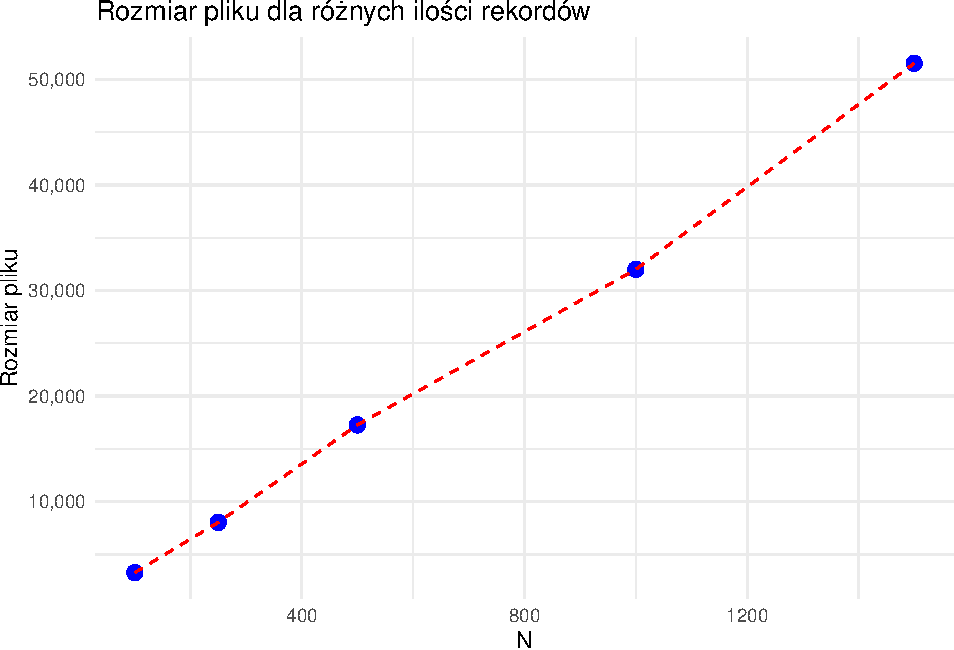
\includegraphics{sbd1_files/figure-latex/unnamed-chunk-2-1}

Jak widzimy rozmiar plików rośnie liniowo. Do tego widać zależność
rośnięcia plików blokowo.

\begin{longtable}[]{@{}
  >{\centering\arraybackslash}p{(\columnwidth - 8\tabcolsep) * \real{0.0795}}
  >{\centering\arraybackslash}p{(\columnwidth - 8\tabcolsep) * \real{0.1932}}
  >{\centering\arraybackslash}p{(\columnwidth - 8\tabcolsep) * \real{0.2955}}
  >{\centering\arraybackslash}p{(\columnwidth - 8\tabcolsep) * \real{0.3523}}
  >{\centering\arraybackslash}p{(\columnwidth - 8\tabcolsep) * \real{0.0795}}@{}}
\toprule\noalign{}
\begin{minipage}[b]{\linewidth}\centering
alpha
\end{minipage} & \begin{minipage}[b]{\linewidth}\centering
rozmiar indeksu
\end{minipage} & \begin{minipage}[b]{\linewidth}\centering
rozmiar obszaru głównego
\end{minipage} & \begin{minipage}[b]{\linewidth}\centering
rozmiar obszaru przepełnienia
\end{minipage} & \begin{minipage}[b]{\linewidth}\centering
Suma
\end{minipage} \\
\midrule\noalign{}
\endhead
\bottomrule\noalign{}
\endlastfoot
0.3 & 2192 & 43840 & 2880 & 48912 \\
0.4 & 1164 & 33280 & 2720 & 37164 \\
0.5 & 1424 & 28480 & 1760 & 31664 \\
0.6 & 1152 & 23040 & 2240 & 26432 \\
0.7 & 1104 & 22080 & 640 & 23824 \\
\end{longtable}

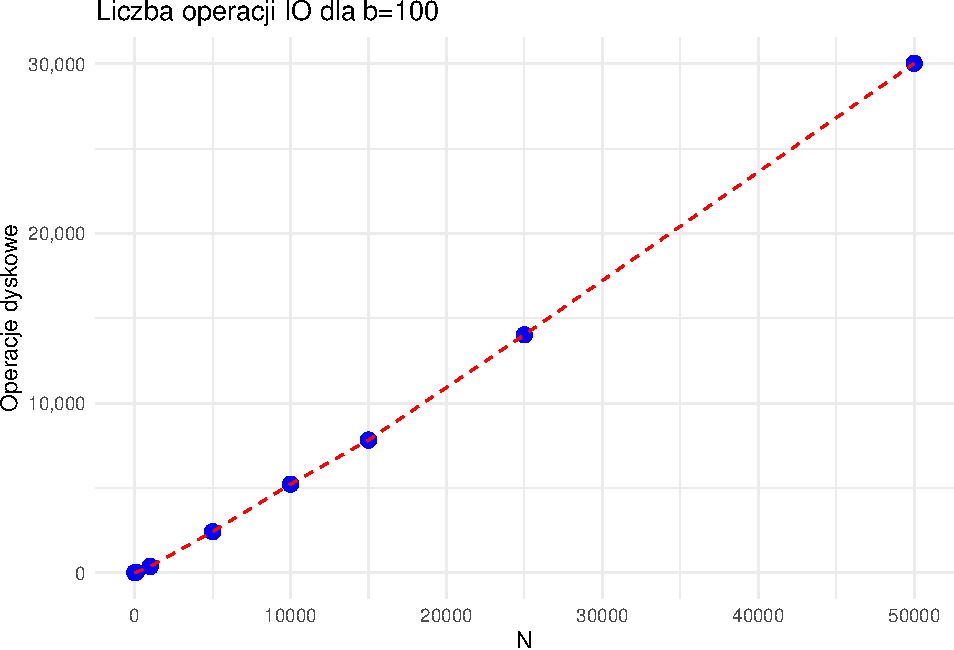
\includegraphics{sbd1_files/figure-latex/unnamed-chunk-3-1}

Widzimy, że spadek rozmiaru pliku jes gwałtowny pomiędzy
\(\alpha=[0.3;0.4]\) oraz później tendencja jest w mniejszym stopniu. To
znaczy, że reorganizacja tworzy mniej stron, przez co będą pełniejsze,
ale reorganizacja będzie musiała następować częściej.

W następnym eksperymencie, dla lepszego zobrazowania danych zmieniłem
wielkość bloku na 10 rekordów.

\begin{longtable}[]{@{}cccc@{}}
\toprule\noalign{}
alpha & śr. odczyty & śr. zapisy & Suma \\
\midrule\noalign{}
\endhead
\bottomrule\noalign{}
\endlastfoot
0.3 & 4.15 & 1.967 & 6.117 \\
0.4 & 4.23 & 1.990 & 6.220 \\
0.5 & 4.21 & 1.990 & 6.200 \\
0.6 & 3.85 & 1.950 & 5.800 \\
0.7 & 4.04 & 1.980 & 6.020 \\
\end{longtable}

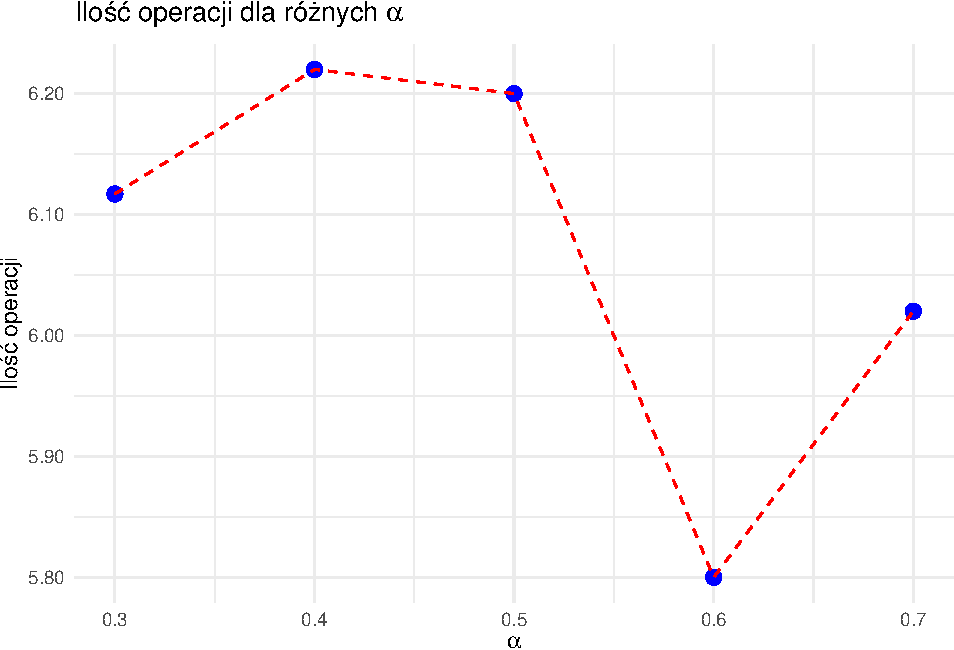
\includegraphics{sbd1_files/figure-latex/unnamed-chunk-4-1}

Widzimy że operacje oscylują w okolicy liczby \(6\). Zapisy zawsze są
blisko \(2\), a odczyty blisko \(4\). Ilość odczytów głównie zależy od
tego jak bardzo porozrzucane są następne elementy w łańcuchu
przepełnień, na co głównie wpływ ma duża losowość.

\section{Podsumowanie}\label{podsumowanie}

Projekt pozwolił na zrozumienie organizacji indeksowej pliku i dlaczego
indeksowanie pozwala znacząco przyspieszyć wszystkie typy operacji, oraz
korzyści płynące z posiadania indeksu. Na bazie eksperymentów, można
zuważyć zależności pomiędzy \(\alpha\) oraz wielkością pliku i ilością
operacji.

\end{document}
